\documentclass[conference]{IEEEtran}
\IEEEoverridecommandlockouts
% The preceding line is only needed to identify funding in the first footnote. If that is unneeded, please comment it out.
\usepackage{cite}
\usepackage{amsmath,amssymb,amsfonts}
\usepackage{algorithmic}
\usepackage[pdftex]{graphicx}
\usepackage{textcomp}
\usepackage{xcolor}
\usepackage{verbatim}
\usepackage{hyperref}
\usepackage{array}
\usepackage{helvet}
\renewcommand{\familydefault}{\sfdefault}
\pdfcompresslevel=9
\pdfobjcompresslevel=3
\def\BibTeX{{\rm B\kern-.05em{\sc i\kern-.025em b}\kern-.08em
    T\kern-.1667em\lower.7ex\hbox{E}\kern-.125emX}}
\begin{document}
\renewcommand{\figurename}{Figure}


\title{Breaking the Linear Barrier: A Multi-Modal LLM-Based System for Navigating Complex Web Content}

\author{\IEEEauthorblockN{Gabriel Moterani}
\IEEEauthorblockA{\textit{Digital Innovation Lab} \\
\textit{Faculty of Computer Science and Technology} \\
\textit{Algoma University}\\
Brampton, Canada \\
gamorimmoterani@algomau.ca}
\and
\IEEEauthorblockN{Wenjun (Randy) Lin}
\IEEEauthorblockA{\textit{Digital Innovation Lab} \\
\textit{Faculty of Computer Science and Technology} \\
\textit{Algoma University}\\
Brampton, Canada \\
randy.lin@algomau.ca}
}

\maketitle

\begin{abstract}
Visually impaired users still face fundamental obstacles when interacting with complex, dynamic websites. Conventional screen readers expose pages in a strict linear order, offer little semantic context for visual media, and provide limited context regarding the page content. This paper introduces a multi-modal accessibility framework combining Large Language Models (LLMs), Computer Vision, and dynamic DOM manipulation to significantly enhance semantic clarity, non-linear navigation, and interaction richness. By interpreting visual and textual web content contextually and adapting it into an intuitive, conversationally navigable interface, our method provides a foundation for visually impaired users to interact effectively with previously inaccessible or challenging digital experiences.

The deployment of a functional prototype on a modern web browser illustrates the capability of the proposed system to interact with diverse websites and tasks. The research team selected Canada's most frequented websites to assess the system's efficacy in enhancing contextual understanding of the page content and enabling navigation through pages and actions via a chat-driven interface. A comprehensive demonstration was executed using a prominent ticketing site, which facilitated users in obtaining a deeper understanding of the page while guiding them towards the successful purchase of concert tickets. By illustrating how vision language and LLM reasoning can be coupled with low‑level browser control, this work lays the groundwork for future efforts in performance optimization, large‑scale evaluation, and personalization across diverse web contexts.
\end{abstract}

\begin{IEEEkeywords}
Web Accessibility, LLM, Accessibility DOM, Human-Computer Interaction, Context-Aware Systems
\end{IEEEkeywords}

\section{Introduction}\label{intro}

Web accessibility has posed a significant challenge to developers since the inception of web browsers capable of rendering HTML markup into visual pages. The evolution of technology has led to the development of systems such as screen readers, which convert the parsed content into audio descriptions. These descriptions are derived from the interpretation of the website's code. With the increasing adoption of the internet and advancements in modern browser capabilities, innovative techniques have been devised, enabling developers to produce code that enhances both screen-reader capabilities and navigation for users with visual impairments. The World Wide Web Consortium (W3C) was established as a consortium to define standards for the advanced implementation of the internet. While addressing multiple concerns, the organization has proposed standards that are continually evolving to enhance the user experience for individuals with impairments. The Web Content Accessibility Guidelines (WCAG), established in May 1999, provide the foundational guidelines that developers should integrate into their code to improve communication with accessibility tools. Nevertheless, although these guidelines hold the potential to enhance user experience, studies indicate a low (or poor) adoption of these practices. \cite{abuaddous2016web, antonelli2018survey} 

These challenges persist even as awareness and technological capabilities have advanced. In particular, 88\% of the websites on the World Wide Web are still not accessible, reflecting a persistent gap between inclusive design principles and their real-world application. \cite{webaccess2024, martins2024large}

Despite the existence of technologies to convert text into audio and to provide a good navigation experience for impaired users, reality shows that navigating the web could be still a challenge for the average impaired person. Another reason for this disconnect lies in the limitations of traditional assistive tools such as screen readers. These systems rely on linear textual content interpretation, which struggles with the complexity and interactivity of modern web experiences, particularly on platforms that depend on multimedia content, multi-step forms, or dynamically updated dashboards. Compounding the issue is the inconsistent implementation of accessibility standards such as the WCAG, most recently updated with WCAG 3.0 in 2024. Although these guidelines offer a robust framework for accessible design, their application often falls short due to a lack of developer expertise, improper use of ARIA (Accessible Rich Internet Applications) tags, and a prevailing focus on visual aesthetics rather than semantic clarity. \cite{gbd2021, wcagchallenges2025}

Recent advances in context-aware technologies, including Large Language Models (LLM), Computer Vision, and Machine Learning, present new opportunities to narrow the accessibility gap. These technologies can augment traditional assistive devices by functioning as intelligent agents, capable of real-time interpretation, restructuring, and interaction with web content. They facilitate the creation of alternative contexts within the accessibility framework, enabling effective content rendering in audio readers and fostering new modes of Internet interaction for users with various impairment issues, such as motor disabilities. Such systems can dynamically adapt interfaces to align with users' goals, offering not only improved content understanding but also richer forms of interaction.

In this study, we introduce a browser-based accessibility framework driven by a multi-modal architecture that synergies vision-language reasoning, contextual manipulation, and dialogue-based task planning. Our framework is realized as an extension compatible with prominent web browsers such as Google Chrome, Safari, and Firefox, on both desktop and mobile platforms. Furthermore, it augments the structural and semantic aspects of web content. This system operates collaboratively across the Document Object Model (DOM) and the browser's Accessibility Tree, equipping visually impaired users with enhanced capabilities for more efficient browsing, comprehension, and interaction with web content.

The subsequent sections of this paper are structured as follows: \autoref{review} undertakes a review of related work and accessibility technologies; \autoref{system} elucidates the proposed system along with its modular architecture; \autoref{methodology} explicates the implementation methodology; \autoref{demo} illustrates a practical usage scenario that demonstrates the system's functionality; \autoref{test} discusses the results obtained from testing the application across a selection of frequently accessed websites, thereby providing insights into the effectiveness of the proposed system; and \autoref{conclusion} concludes with considerations, limitations, and suggestions for future research directions.


\section{Literature Review}\label{review}

Multiple studies in the past two decades have documented how screen readers process web pages strictly in a linear sequence, forcing visually impaired users to traverse headings, menus, and decorative elements before reaching relevant content. \cite{Ramakrishnan2017-rn, wcagchallenges2025, martins2024large, abuaddous2016web} Large‑scale audits continue to report widespread keyboard navigation barriers, even on sites that advertise compliance with the success criteria in WCAG 2.x and the draft of WCAG 3.0 for 2024.\cite{wcagchallenges2025}

Empirical user observations show that the absence of semantic grouping leads to excessive keystrokes and cognitive overload when interacting with dashboards, multi‑column news layouts, and e‑commerce grids. Despite incremental improvements in screen reader software, the underlying linear traversal model remains unchanged, leaving the fundamental navigational burden on the user. \cite{ferdous2021semantic}

When browsing the internet, users without impairments can efficiently skim through and scan texts, thereby saving time and disregarding irrelevant information. In contrast, individuals who depend on screen-readers and other accessibility tools are deprived of this ability. Consequently, such users must often listen to a substantial portion of content to determine whether to continue seeking information on a particular website. \cite{Ramakrishnan2017-rn} This situation underscores that, despite the increased adoption of relevant guidelines and technological advancements, a more contextual and dynamic approach should be pursued.

Accessible design guidelines require developers to provide meaningful alternative text, ARIA roles, and programmatic relationships, but field surveys reveal that these elements are missing or optimized for search engine ranking rather than human comprehension. \cite{wcag2023} Where alt text is present, it is often terse ("image1") or redundant with surrounding captions, providing little help in grasping complex visuals such as charts, info-graphics, or hero banners. Even on sites that partially implement WCAG techniques, dynamic content injected by third‑party ad networks or CMS templates escapes validation, breaking reading order and semantic context. \cite{wcagchallenges2025} As a result, visually impaired users must infer meaning from fragments that were never authored with their experience in mind.

Recent prototypes illustrate how LLM, computer vision, and DOM automation can enrich accessibility beyond traditional screen readers. Commercial and research extensions now parse shopping pages to surface product attributes in a simplified view, reducing navigation steps. \cite{prakash2024} Task‑oriented agents powered by LLMs translate natural‑language commands into browser actions, demonstrating promise in filling out forms, filtering tables, or performing multi‑step tasks. \cite{he2024webvoyager} While these systems validate the feasibility of AI‑mediated assistance, they remain domain specific, rely on brittle heuristics, or lack an integrated mechanism for maintaining conversational context across page transitions.\cite{kodandaram2024,mehendale2024}

Principal investigations are concentrated on employing a visual compiler methodology, wherein the context derived from 'screenshots' serves as the primary element for parsing page content, facilitating alterations to the webpage, or enabling user navigation with the support of auxiliary LLM tools. Although screenshots offer a comprehensive understanding of the page's context, LLMs interact with textual data, establishing a paradigm in which their application is not optimized for textual analysis. The primary applications proposed herein is deficient in its capacity to integrate seamlessly into the conventional workflow of an internet user. As an independent application, while it addresses certain aspects of the problem, it simultaneously engenders a new challenge by eschewing the utilization of browsers as its principal mechanism. \cite{he2024webvoyager, mehendale2024, prakash2024}

\subsection*{Synthesis and Identified Gaps}

Taken together, the literature confirms that technical progress has not yet resolved several critical barriers:

\begin{enumerate}
\item \textbf{Non‑linear navigation is still unsupported.} Screen readers continue to expose content in a purely sequential manner, forcing users through irrelevant elements before they reach task‑relevant information. \cite{Babu_2013} 
\item \textbf{Semantic context for visual content is insufficient.} Alt text and ARIA labels are inconsistently authored, providing at best superficial descriptions that fail to convey rich visual meaning. \cite{Chintalapati_2022}
\item \textbf{General‑purpose, task‑driven interaction remains elusive.} AI‑augmented tools demonstrate success in narrow domains but do not yet offer a unified solution for complex, cross‑site workflows.\cite{prakash2024,kodandaram2024,mehendale2024} 
\end{enumerate}

Addressing these gaps requires a comprehensive approach that builds upon existing assistive technologies while introducing innovative solutions. Our work focuses on developing a system that leverages the widespread adoption of screen readers and browser extensions among Blind and Vision Loss (BLV) users. By combining established accessibility tools with advanced AI capabilities, we aim to create a more adaptive and intuitive navigation experience.Our approach is further distinguished by employing browsers as the primary framework for developing functionalities that seamlessly integrate with the existing workflow of users, thereby facilitating adoption and enhancing the ease of website interaction. 

This methodology integrates multiple layers of assistance: enhancing semantic understanding through improved content interpretation, providing context-aware navigation options, and enabling task-oriented interactions through natural language processing. The resulting system seeks to bridge the gap between traditional accessibility tools and modern web interfaces, offering BLV users a more seamless and efficient way to interact with complex web content.

\section{Proposed System Overview}\label{system}

While browsing the Internet, users rely on software applications capable of facilitating data exchange with cloud servers via the Hypertext Transfer Protocol (HTTP), ultimately acquiring Hypertext content formatted in Hypertext Markup Language (HTML). These applications convert the textual representation of web pages into a visual format. These software applications are denominated as web browsers. Currently, Google Chrome constitutes the primary browser used within desktop environments, accounting for a 66\% market share. In contrast, Safari is used predominantly on mobile platforms used by 22\% of mobile users.\cite{browserstats2025}

Web browsers have evolved to facilitate applications that function in conjunction with the product through the use of browser APIs. These applications, known as extensions, are installable within browsers and serve to augment the overall capabilities of the browser. Extensions enable developers to create enhancements for standard navigation, facilitating features such as text grammar correction, ad blockers, and other mechanisms. In this project, extensions are employed to interact with the DOM, which is the technical representation of elements on a web page in browsers, as well as the Accessibility Tree, which shares the same representation but is focused on what screen readers (SR) mechanisms utilize to convert content for visually impaired users.

As shown in \autoref{tab:architecture}, our architecture orchestrates four cooperative modules around a shared task graph and state log. The LLM serves as the reasoning core, translating between raw pixels/DOM, natural language dialog, and low-level interaction events.

\subsection{Visual‑Layout Interpreter (VLI)}

The VLI system acquires periodic snapshots of Document Object Model (DOM) elements, analyzing the content through various methodologies to construct a JavaScript Object Notation (JSON) representation of a website's elements. This JSON representation undergoes further analysis to extract images, textual content, interactive actions, advertisements, navigational content, and also to identify WCAG infringements. In essence, the VLI is tasked with the collection and conversion of webpage elements into a technical format that facilitates modification and interaction by other modules within the application. A simplification of this module can be inferred from \autoref{fig:vli}.

\begin{figure}[h]
\centering
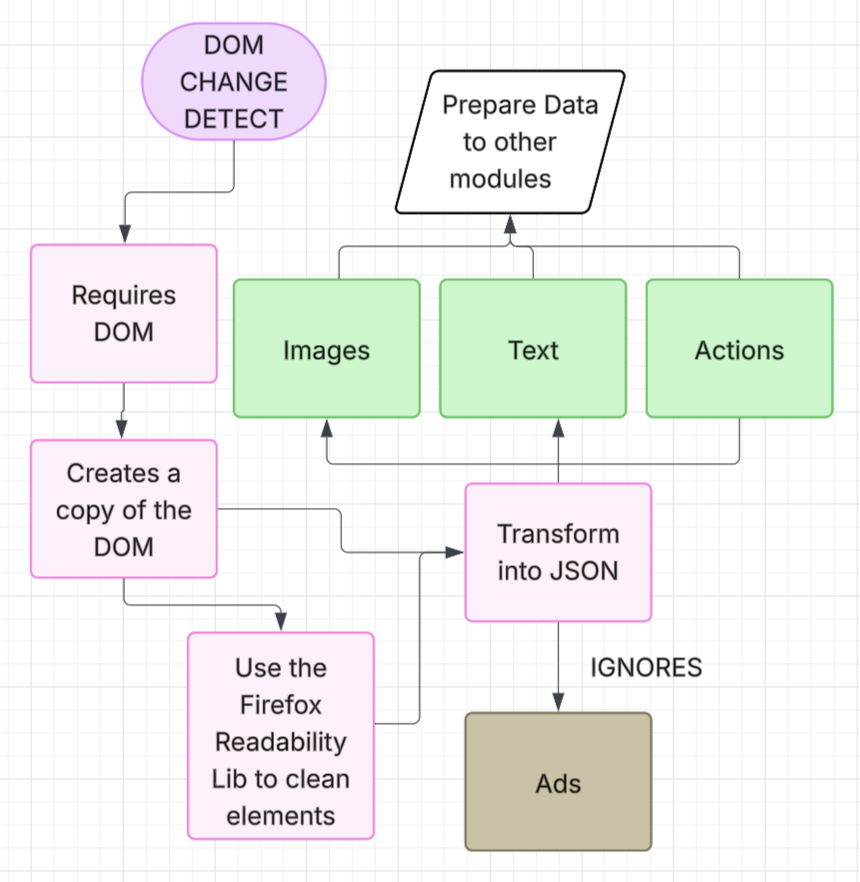
\includegraphics[width=\columnwidth]{images/VLI.png}
\caption{Simplification of VLI module.}
\label{fig:vli}
\end{figure}


\subsection{Contextual Modification Engine (CME)}

As demonstrated in \autoref{fig:cme}. The CME works as an orchestrator for the application, it consumes, text, images, actions, and WCAG infringements created by the VLI to use multiple techniques to contextually parse the content, acting as the main engine for the other modules. After receiving data, the CME will interact with the backend to receive a summary of the page, and to require for each image provided that has no adequate alternative text a new content improving the context of the overall pages. A summary of the page is also provided for the user in the top of the page to allow the user to skim and make a decision if the user wants to continue interacting with that webpage. Images alt properties are inserted async providing user the best content without taking time to process all content. Finally, WCAG infringements are parsed by the LLM model trying to find adequate methods to fix the tags to be in compliance with the standards and guidelines, providing a better experience.

\begin{figure}[h]
\centering
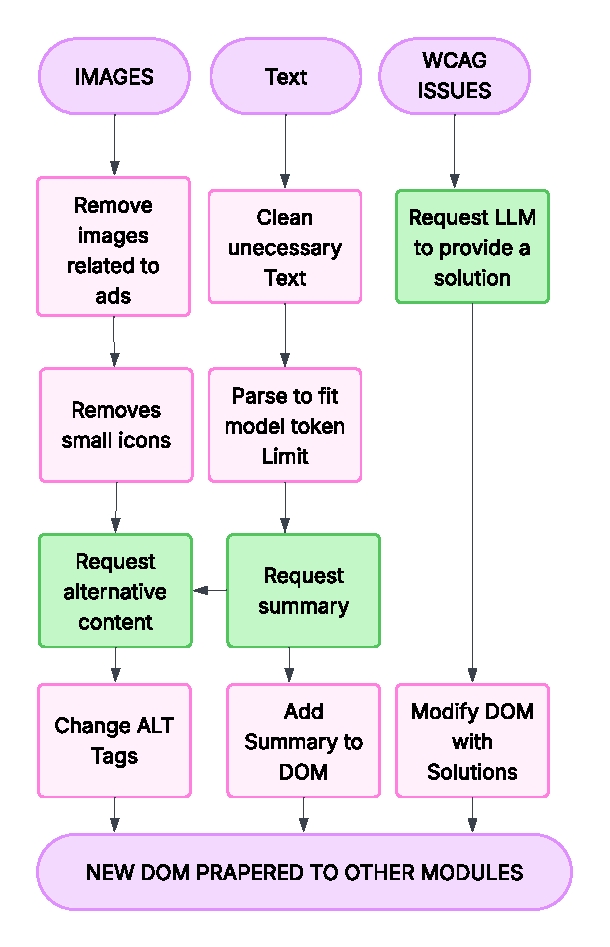
\includegraphics[width=\columnwidth]{images/CME.pdf}
\caption{Simplification of CME module.}
\label{fig:cme}
\end{figure}

\subsection{Conversational Plan Manager (CPM)}

The CPM runs a mixed‑initiative chat: it elicits the user's intent, iterates over the VLI exported actions JSON, and creates reasoning using an LLM model to create a output of actions to be taken to complete each proposed task. The LLM is responsible for understanding each possible action and is responsible for each task as well as what JS command should be triggered to make execute that command. That plan is then used by the multi-modal Interaction Module to execute commands and then complete tasks. A representation of that communication with the back end to acquire reasoning tasks can be verified in \autoref{fig:communication}.

\subsection{Multi-modal Interaction Executor (MIE)}

The MIE methodically progresses through the plan, rigorously evaluating the suggested JS commands, confirming the presence of each proposed interactive element, making necessary adjustments, and ultimately executing the JS commands required to achieve the specified user task.

\begin{table}[h]
\centering
\caption{System Components and Their Roles}
\label{tab:architecture}
\small
\renewcommand{\arraystretch}{1.3}
\begin{tabular}{|>{\raggedright\arraybackslash}p{0.8cm}|>{\raggedright\arraybackslash}p{2.5cm}|>{\raggedright\arraybackslash}p{4cm}|}
\hline
\textbf{Name} & \textbf{Functional Role} & \textbf{Rationale} \\
\hline
\texttt{VLI} & Visual understanding of the current page & Parses the rendered page DOM into a structured semantic graph usable by language and planning components. \\
\hline
\texttt{CME} & Parses content and provide additional context & Communicates with Backend to request additional content modifying page for a better experience. \\
\hline
\texttt{CPM} & Dialogic intent capture \& planning & Conducts a mixed-initiative dialog to clarify the user's objective, decomposes it into an executable plan, and maintains a progress log. \\
\hline
\texttt{MIE} & Autonomous action execution & Carries out the CPM's plan (clicks, typing, drag-and-drop, drawing), and after each step re-invokes the VLI to verify success or recover. \\
\hline
\end{tabular}
\end{table}


\subsection*{Example Workflow}

During the system's development, multiple visually impaired individuals were consulted regarding challenging tasks encountered on the internet. A prevalent issue identified was the navigation of online news sites. Despite developers' attempts to enhance accessibility, the dynamic elements, such as advertisements and diverse news services, render navigation overwhelming and nearly unmanageable. The transient nature of news, coupled with the vast volume of content produced, significantly impedes content adaptation for visually impaired users. 

In this scenario, we are modeling the basic process of accessing a news website to obtain insights regarding the essential conclusions of the most significant articles, as demonstrated in \autoref{tab:sequence}.

\vfill
\begin{table}[h]
\centering
\caption{Phase and Module Sequence}
\label{tab:sequence}
\footnotesize
\renewcommand{\arraystretch}{2}
\begin{tabular}{|c|p{5.5cm}|}
\hline
\textbf{Phase} & \textbf{Module Sequence} \\
\hline
Intent capture & CPM → user: "What would you like to do?" → user: "Read today's headlines." \\
\hline
Context analysis & VLI parses home page; CME adapts headline list. \\
\hline
Plan and Execution & CPM drafts plan, while MIE executes. User navigates to article pages where the VLI presents summary and loop continues\\
\hline
\end{tabular}
\vspace{0.5cm}
\end{table}

\section{Prototype Architecture}\label{methodology}

The proposed system is demonstrated through a prototype system to illustrate navigational capabilities for people with visual impairments. This architecture can be methodically categorized into two primary structures: Front-end Development and Back-end Development, as shown in \autoref{fig:communication}.

The front-end architecture facilitates the interaction between the browser and the tool, involving the extraction of data from the page, its transformation into pertinent nodes, and the establishment of interactions between the system-page and the user-system.

\begin{figure}[h]
\centering
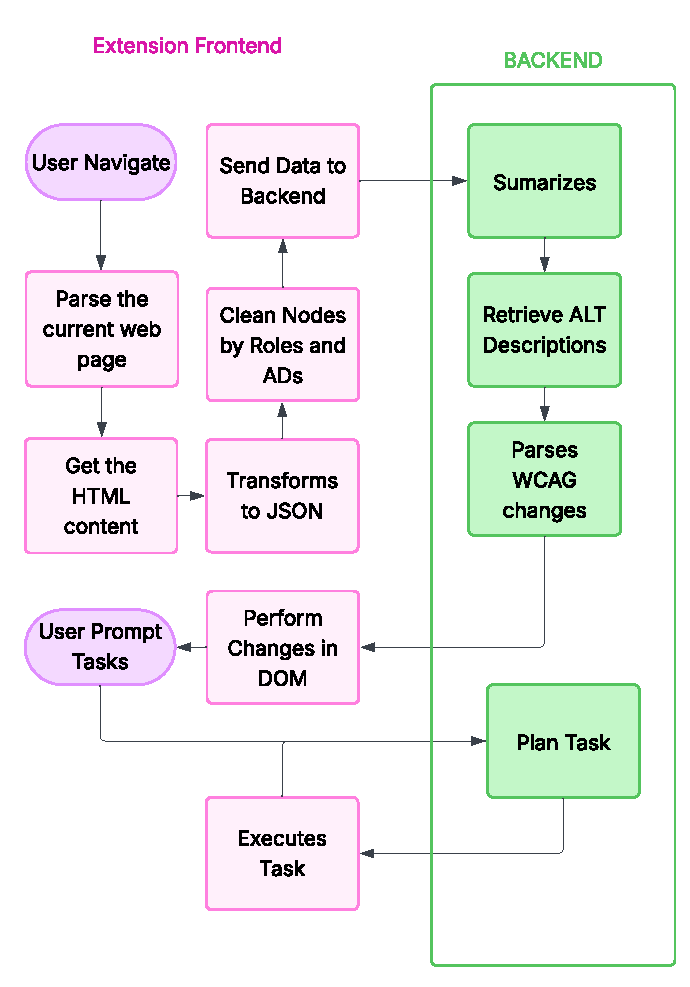
\includegraphics[width=\columnwidth]{images/5.pdf}
\caption{Simplification of the Backend - front-end Communication.}
\label{fig:communication}
\end{figure}

\subsection{Front-end Structure}

In the process of constructing the front-end architecture, a comprehensive investigation into frameworks was undertaken to identify those that would offer enhanced performance and maintainability for the tool, as well as competence in interfacing with browser APIs effectively. The Plasmo framework for web extension development was selected as the foundational technology for the extension's creation. Plasmo integrates the web-ext library to facilitate the development of extensions using Javascript and Typescript languages, enabling the incorporation of sophisticated front-end libraries such as Reactjs. The amalgamation of these technologies enabled developers to craft efficient, streamlined, and consistent interactions among pages, systems, and users.

Upon the rendering of a new page, the front-end system detects alterations in the primary DOM elements, recognizing a modification and thereby activating the designated system to acquire both the DOM and accessibility trees. This process involves filtering out superfluous content utilizing ad blocking technology and a readability library, a JavaScript library specifically designed to enhance readability by removing unnecessary content.

Since the technologies underpinning LLM depend on the volume of input text, which is converted into tokens - the fundamental units of LLM data — it is crucial that the front-end system sanitizes the input to supply the data interpreter with only essential information. Failure to do so requires that the content be divided into smaller segments for processing. This segmentation can result in an increase in the rendering time of contextual elements, higher server costs, and potential loss of context.

To generate a cleaner version of the DOM, an initial pre-processing step was used to exclude advertising-related elements. This was achieved through the application of a set of community-maintained blacklist rules, implemented via a custom reimplementation of a DOM-cleaning library designed to apply these filtering criteria. Following this sanitation phase, the Readability JS library, originally developed by Mozilla for Firefox, was utilized to further refine the DOM by removing nonessential nodes, thereby preserving only the content most relevant to user navigation and comprehension.

Subsequent to the purification of elements, the front-end will extract the main content transforming into a JSON representation, which is more iterable over programming languages than the pure DOM representation. This JSON is iterated over to extract main components that will be the input of each module described in the previous sections. A new representation is created with the actions, texts, images, and tags with WCAG violations.

Finally, front-end establish communication with the back-end modules through fundamental HTTPS requests using the fetch library. These modules will furnish the requisite context and information to be elaborated upon in the back-end subsection of this section. The front-end will then transform this contextual information into DOM modifications aimed directly at engaging with the Accessibility Tree, thereby enhancing the end-user experience. Furthermore, the extension will inject HTML elements into any web page, facilitating user interaction with the extension system, thereby enabling effective user-system communication and task execution by the system on behalf of the user.

\subsection{Back-end Structure}

The backend system is comprised of a dockerized Flask Python server configured to receive messages on a web accessible endpoint. These messages are processed and converted into executable tasks for the system, resulting in outputs that are subsequently utilized by the front-end in response to the queried messages. 

Although the back-end encompasses a variety of techniques, it is essential to articulate four principal modules to provide clarity regarding its functionality.

\subsubsection{Visual Computation Methodology}

The backend component is tasked with receiving all visual elements, which may include binaries, image URLs, CSS (Cascading Style Sheets) cascade elements, or any other elements that pertain exclusively to a visual context. Based on the specific format of each element, the system processes these into images that are forwarded to a Computer Vision Machine Learning System. This system employs an algorithm that has been trained with an extensive dataset comprising billions of images, enabling it to accurately identify and describe the content within the images. The resulting image description is synthesized with a summary generated by an AI (Artificial Intelligence) language model, along with the proximate elements, to provide a comprehensive contextual description of the visual element.

\subsubsection{Context Aware Methodology}

This component is responsible for receiving text, processed, and queried by the front-end from the DOM. This text is transmitted in JSON format and encompasses both the page content and the type of HTML tag encapsulating the text. The server then processes this information using a Large Language Model system, which extracts both the summary and additional context from the page. This refined information is subsequently utilized across various Back-end and Front-end modules throughout the system's operational workflow.

\subsubsection{WCAG Compliance Methodology}

The component receives a JSON representation of DOM elements that violates WCAGs rules, upon which it processes these data through a finely tuned Large Language Model system. This LLM has been trained using data from websites that are exemplary of effective and ineffective adherence to the WCAG guidelines. Consequently, the LLM returns a JSON containing element identifiers and suggestions for compliance modifications or new tags. These modifications facilitate the conversion of the website's accessibility framework into a format that can be accurately interpreted by TTS systems. The front-end is then responsible for elucidating this information and, accordingly, transforming the page.

\subsubsection{Conversational Task Executer Methodology}

Following the primary execution phase for context preparation, the server promptly stores an available action representation of the visited website. This object facilitates rapid and efficient communication with the AI, which is powered by an LLM. The content is queried via LLMs, enabling the identification of specific portions of the HTML code necessary for various tasks solicited by users. Afterward, it returns executable actions via JavaScript. The front-end, equipped with this information, utilizes JavaScript commands to perform tasks on behalf of visually impaired users.

\section{Prototype Demonstration}\label{demo}

The presented example workflow aims to elucidate a straightforward task that can be performed by any user seeking to obtain fundamental information regarding the acquisition of tickets to a concert. In this prototype demonstration, we will simulate the challenges faced by a visually impaired individual in comprehending the available concerts on a relevant ticket website. Following installation of the Google Chrome extension, the DOM elements will undergo modification, resulting in alterations to the accessibility tree, as illustrated in \autoref{fig:start}.

\begin{figure}[h]
\centering
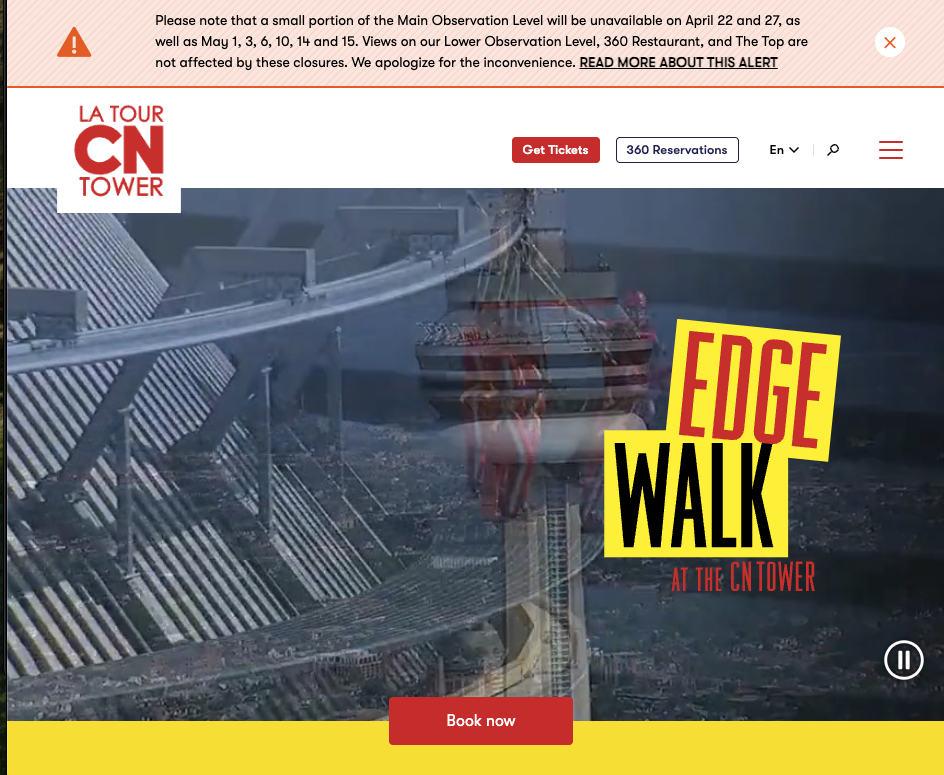
\includegraphics[width=\columnwidth]{images/1.png}
\caption{Page is loaded and system start parsing content}
\label{fig:start}
\end{figure}


Humans possess the ability to scan and skim web pages, allowing them to assess the relevance of the page and the accuracy of the information before engaging in the full content. This seemingly straightforward human skill is often absent among BLV users. When a website is accessed using the extension, the initial task for the system is to generate a summary of the page. This summary facilitates the user's decision-making process regarding the potential navigation of the site. Ideally, the summary should be prepared within the standard Large Contentful Paint (LCP) average time of three seconds. This enables users to make an informed choice about engaging with the page and provides the interface necessary for interaction.

\begin{figure}[h]
\centering
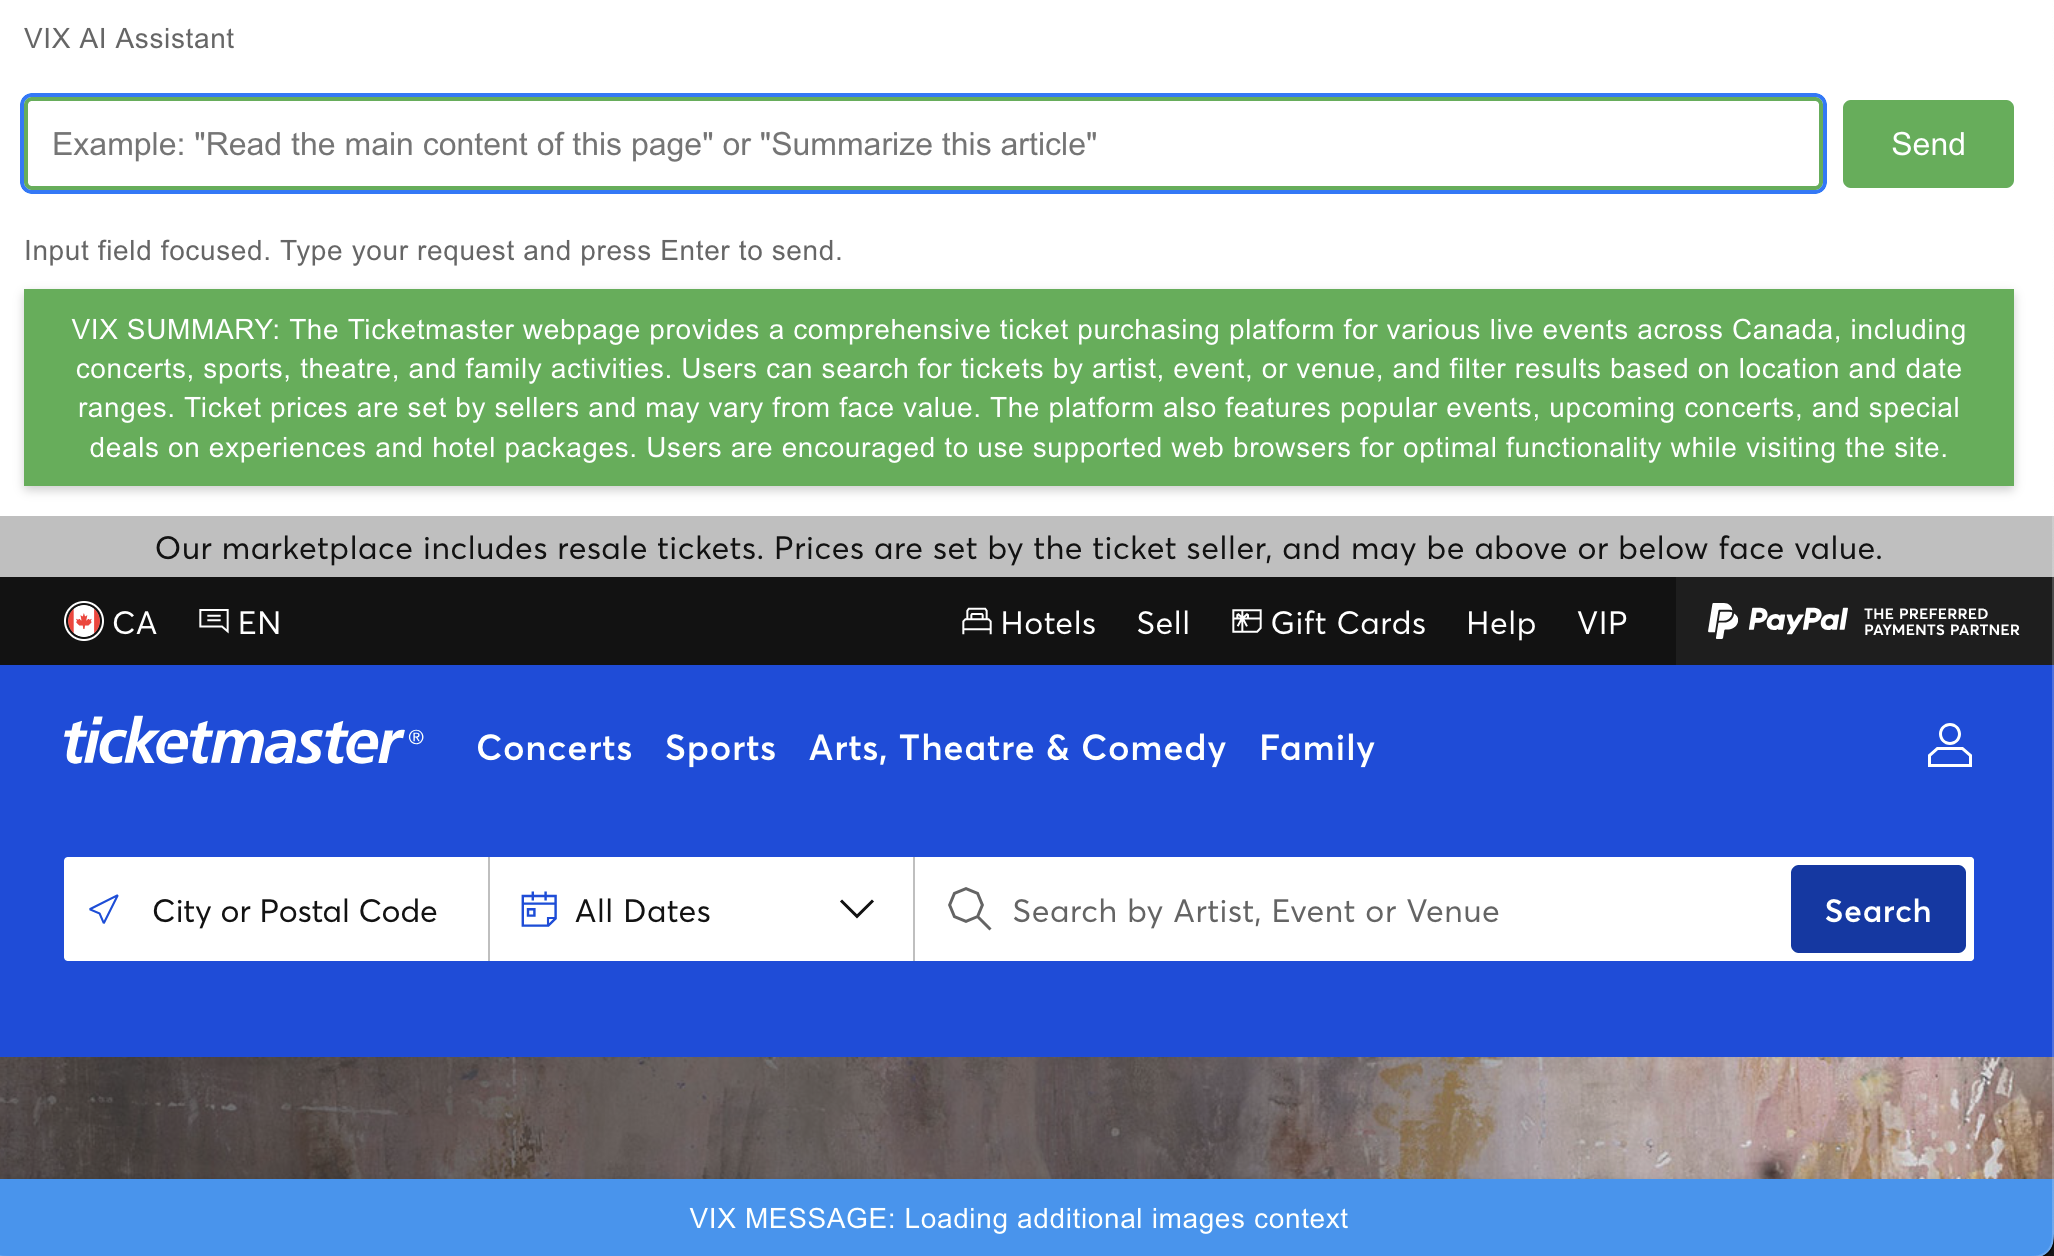
\includegraphics[width=\columnwidth]{images/2.png}
\caption{Summary and Chat Interfaces displayed}
\label{fig:chat}
\end{figure}

\autoref{fig:chat} provides a visual demonstration of the elements inserted in the accessibility tree to be used by screen readers to deliver the new content to BLV user. After the manipulation of the DOM elements into a summary and a chat interface the system continue asynchronously to work in the effort to manipulate HTML to be WCAG compliance.

This process employs the axe-core JavaScript library to identify tags and images that do not comply with WCAG standards. The backend system then iterates over these elements to generate the missing attributes or enhance attributes that remain non-compliant. Following communication with the back-end, the front-end proceeds to adjust the webpage to ensure that the end user can navigate effectively, notwithstanding the incomplete implementation of accessibility features.

\begin{figure}[h]
\centering
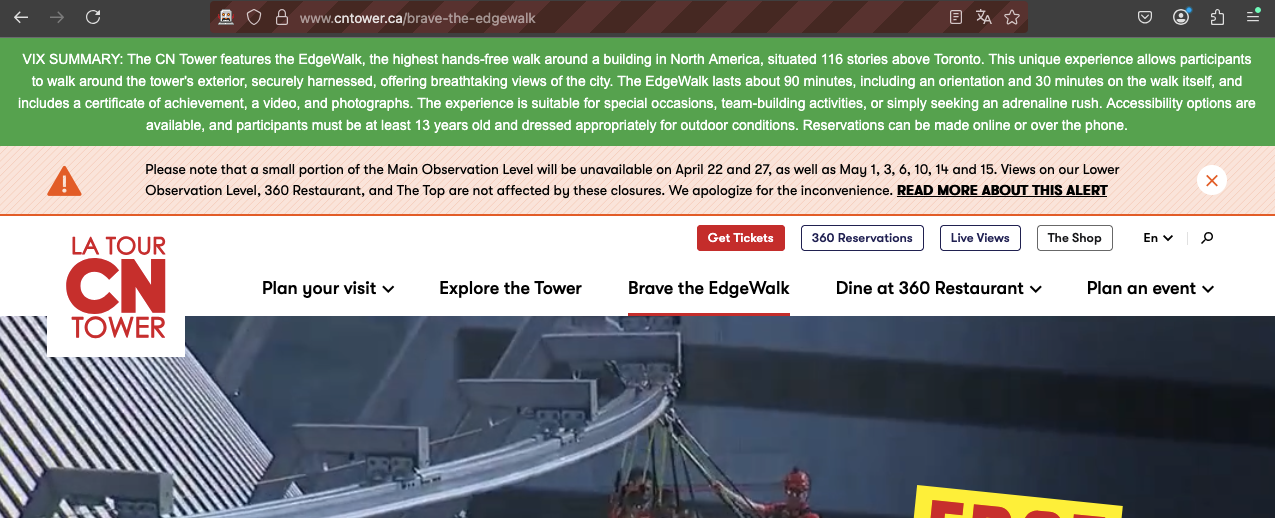
\includegraphics[width=\columnwidth]{images/3.png}
\caption{Image and it's alternative text created by LLM}
\label{fig:alt}
\end{figure}

\autoref{fig:alt} illustrates an image extracted from the website, for which the extension retrieved a novel alternative description that would otherwise be inaccessible to the BLV user, rendering it invisible to them. Such content has the potential to enhance the user's navigational experience if the end user deems it beneficial.

User can now interact with the page either using it's own navigation or by chatting with the tool, prompting the system to perform actions on it's behalf. In this demonstration, the user prompted the AI to buy tickets to the Bryan Adams concert. After analyzing the DOM elements, the accessibility tool then clicked in the link (using JS actions) related to that concern, navigating user to a new page where the journey repeats itself.

\begin{figure}[h]
\centering
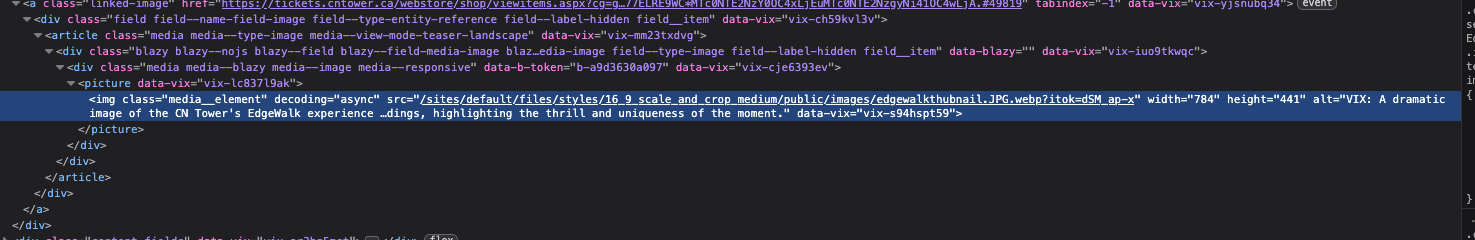
\includegraphics[width=\columnwidth]{images/4.png}
\caption{Page navigated after the AI prompted}
\label{fig:show}
\end{figure}

As shown in \autoref{fig:show}, the system successfully facilitated user navigation to a new page, where now users need to select seats and perform payment. It is imperative to consider that in subsequent versions of this application, the CPM should be capable of continue executing tasks on new pages to ensure the continual achievement of the targeted user objective. Due the time constrains the team yet not developed the continuously loop over tasks and pages. Being part of the scope for future implementations.


\section{Tests \& Findings}\label{test}

Previous studies underscore that the primary challenge inherent in these technologies lies in demonstrating their effectiveness across a wide array of web page contexts. \cite{prakash2024, he2024webvoyager} To evaluate and confirm the efficacy of the application, the authors decided to implement the extension on the 10 most accessible websites in Canada (as reported by SemRush).\cite{semrumsh} Furthermore, a selection of additional websites outside the most visited rankings was incorporated to provide a more comprehensive perspective. The enumeration of these websites is available in \autoref{tab:results}.


\begin{table*}[ht]
\centering
\caption{Extension Analysis Key Results for Each Website}
\label{tab:results}
\small
\renewcommand{\arraystretch}{1.3}
\begin{tabular}{|>{\raggedright\arraybackslash}p{2.5cm}|>{\raggedright\arraybackslash}p{2.5cm}|>{\raggedright\arraybackslash}p{1.8cm}|>{\raggedright\arraybackslash}p{2.5cm}|>{\raggedright\arraybackslash}p{1.5cm}|>{\raggedright\arraybackslash}p{1.5cm}|>{\raggedright\arraybackslash}p{2cm}|}
\hline
\textbf{Website} & \textbf{Category} & \textbf{Monthly Access} & \textbf{HTML Size} & \textbf{Number of Images} & \textbf{WCAG Violations} & \textbf{Efficacy \%} \\
\hline
Wikipedia & Information & 1.36M & 140,852 & 23 & 4 & 80 \\
\hline
Amazon & Shopping & 153M & 948,050 & 238 & 53 & 100 \\
\hline
CBC & News & 2M & 224,808 & 35 & 5 & 40 \\
\hline
Yahoo & News & 235M & 757,533 & 17 & 16 & 0 \\
\hline
NHL & Sports & 11M & 422,463 & 88 & 81 & 60 \\
\hline
Realtor & Services & 34M & 75,189 & 33 & 51 & 20 \\
\hline
Weather & Information & 769M & 1,138,290 & 8 & 23 & 100 \\
\hline
Apple & Shopping & 188M & 302,077 & 0 & 3 & 100 \\
\hline
Indeed & Services & 24M & 399,086 & 2 & 1 & 40 \\
\hline
BMO & Banking & 300K & 2,452,943 & 368 & 0 & 80 \\
\hline
\end{tabular}
\end{table*}

Each website was accessed five times and the data was collected accordingly. A summary of the most relevant data is available in \autoref{tab:results}.
\begin{itemize}
    \item \textbf{HTML Size} (Counted by number of characters in HTML)
    \item \textbf{Number of Images} (Counted by number of individual images)
    \item \textbf{WCAG violations} (Counted by number of number of WCAG rules infringements) 
    \item \textbf{Efficacy} (Calculated by the \autoref{math:eficacy} - Defines the efficacy of the proposed system to complete a task)
\end{itemize}

The efficacy of the system is calculated by the number of times the main task was completed. The main task is defined as the task that the user asked the system to complete. For each website a task was created that matches their main activity (As an example, BMO, a banking system, the tasks provided were: "Help me open a new bank account". The system is considered to have completed the task if the user is able to enter the web page related to the prompted task, or fill the forms related to the same task.

The efficacy is calculated using the \autoref{math:eficacy}:

\begin{equation}
    \label{math:eficacy}
    Efficacy = \frac{Completion}{Attempts}\times 100
\end{equation}

The summary of the results collected during the tests can be checked in \autoref{tab:results}. When analyzing the results while using the application we could notice an improvement of the auxiliary navigation, and also the increase of context provided by the images text alternative property. Especially in websites with large use of images such as BMO. Some websites still insist in the use of non-parsable techniques to reproduce images like apple using SVG and majorly animations and videos, making it impossible to parse the content. However, their good use of the implementation of the WCAG guidelines could provide a good experience, translated into the capacity of the system to execute the prompted tasks.

Upon evaluating, solely moderate to weak associations were discernible between the implementation of WCAG guidelines on a website and the system's capacity to execute tasks. As evidenced in \autoref{fig:violations}, there is a moderate correlation between the number of accessibility errors on websites and the capability to complete tasks. This indicates that websites with superior accessibility are more readily comprehensible and processable by LLM systems to accomplish tasks. Although our system endeavors to address these issues, at the preliminary stages of implementation, it can still be inferred that adherence to these guidelines will enhance efficacy.

\begin{figure}[h]
    \centering
    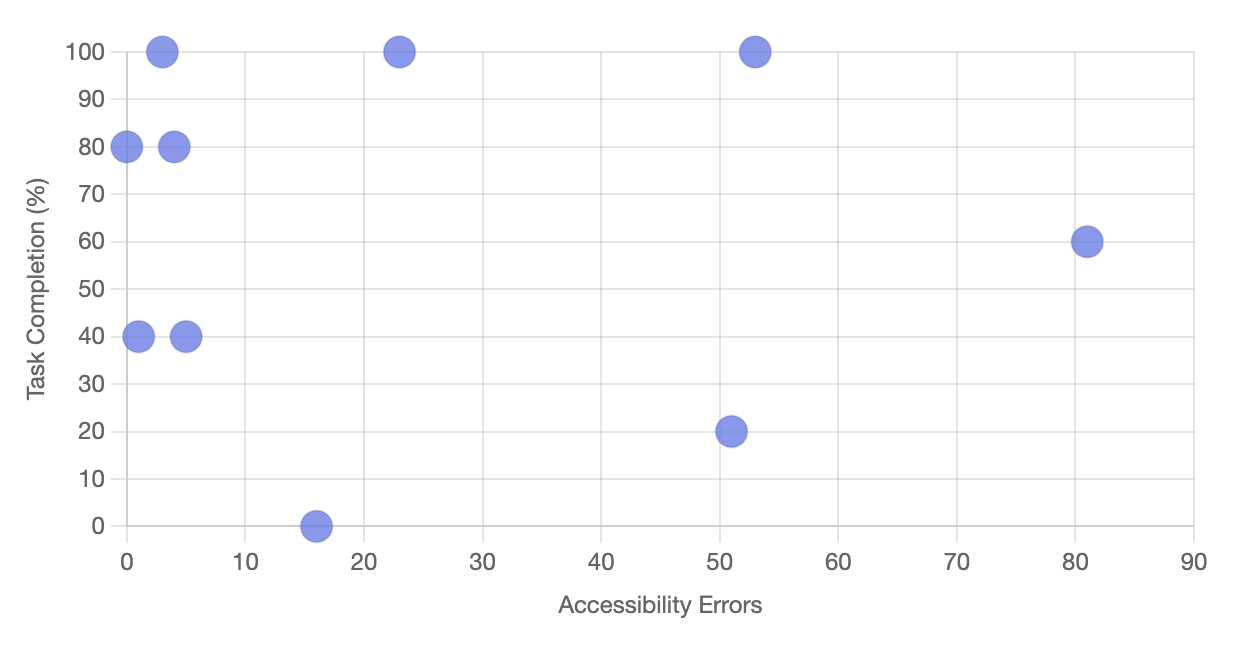
\includegraphics[width=1\linewidth]{images/eficiencexerrors.png}
    \caption{Efficacy x WCAG violations}
    \label{fig:violations}
\end{figure}

\autoref{fig:Complexity} illustrates another correlation, namely the relationship between website complexity, quantified by the number of characters constituting the HTML, and task completion efficacy. Websites with increased content can pose a challenge for LLM systems, particularly due to the requirement for greater processing power to engage with extensive content. While larger website sizes may represent a potential issue, the techniques employed in this prototype effectively distill the necessary content, thereby reducing the data volume transmitted to the model. Additionally, more complex websites offer greater interactivity opportunities and provide more contextual information to their interactive elements, which can enhance the environment for task completion.
\begin{figure}[h]
    \centering
    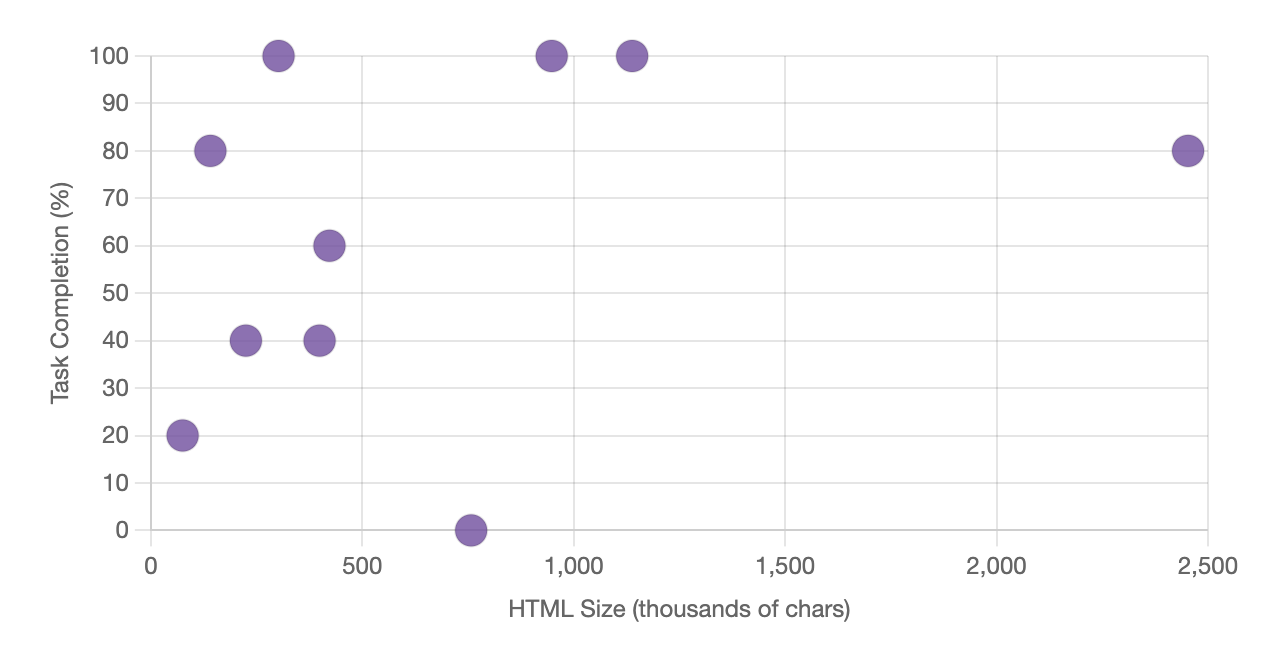
\includegraphics[width=1\linewidth]{images/efficiencexcomplexity.png}
    \caption{Efficacy x Website HTML Size (Complexity)}
    \label{fig:Complexity}
\end{figure}

During tests, developers could notice that fine-tuning the models can be necessary due to the hallucinations that the LLM model is susceptible to. In addition, developers could understand the correlation of the different types of data and how to increase the LLM capability to understand the context. 

For the purposes of this study, the developers opted to employ the GPT 4.1 model, due to its speed and ease of implementation. The utilization of OpenAI SDKs facilitated a straightforward deployment of the LLMs model; however, it also introduced a challenge owing to the company's imposition of restrictions on the number of tokens processed per minute, which are dependent on the account tier of the organization. As our organization is categorized under tier 1, we were constrained by a limit of 200,000 tokens per minute, thereby posing a challenge to reduce the volume of data submitted to the model with each instance. For future research, developers recommend experimentation with alternative models, as well as an enhancement of the organization's tier status, to fully leverage the tool's capabilities.
\section{Conclusion}\label{conclusion}

This paper has addressed critical and persistent accessibility challenges experienced by impaired users navigating web. Through integrating advances in LLMs, computer vision, and dynamic DOM manipulation, we introduced a multi-modal accessibility system designed as a browser extension to significantly enhance web interaction experiences for visually impaired users.

Our architecture uniquely combines four core modules as the VLI, CME, CPM, and MIE to collaboratively parse visual and semantic content, dynamically reorganize web page structures, extract main elements, conduct intent-based conversational planning, and automate complex web interactions. The prototype demonstration using the Ticketmaster's webpage highlighted the system's practical capability to simplify complex navigation tasks, enhance semantic comprehension through improved alt text and ARIA labels, and successfully execute user-driven tasks such as information retrieval and ticket purchases.

The results obtained from dynamic testing involving ten pertinent sites in Canada indicated that while the system exhibits efficiency in task execution, it occasionally manifests hallucinations, leading to incomplete task performance and inaccuracies in modifying the DOM. These findings underscore the need to evaluate additional language models beyond GPT-4.1 and highlight the pursuit of models capable of processing larger datasets and accommodating more extensive contextual information.

However, despite its promising outcomes, several practical and technical limitations have been identified. First, the computational costs associated with real-time inference of LLM and computer vision models remain high, necessitating server resources equipped with high-performance GPUs (Graphics Processing Unit). Second, latency introduced by inter-module communication and iterative page rendering may affect usability during extensive interactions. Third, the prototype's ability to generalize its effectiveness across diverse web structures and complex dynamic websites requires further development and validation. Finally the capacity of the system to navigate multiple web-pages of the same site adding information to the context window, making it more difficult for the system to parse information. 

Future research directions are clear and critical for achieving broader adoption and usability. Optimizing system performance and reducing computational demands through more efficient inference methods and specialized LLM fine-tuning specifically for accessibility tasks are immediate priorities. The research and develop also aims into implementing features like continuously task executer, multi-language contexts and video parser.

Ultimately, while technical innovation forms the core of our approach, the broader vision remains creating a universally accessible internet. Emphasizing user-centered iterative development, ongoing collaboration, and inclusive design principles will ensure that advancements in AI technology translate meaningfully into equitable digital experiences for all users.


\section*{Use of AI Disclosure}\label{ai-disclosure}
No artificial intelligence tools were employed in the generation of the content presented in this document. Throughout the drafting process, the Overleaf AI Assistant was utilized to review grammatical accuracy and to offer feedback on writing style and consistency, thereby suggesting improvements to the text and making modifications to the content. During the coding phase of the project, Claude AI, version 3.5, was employed to assist developers in coding tasks and error resolution.


\section*{Acknowledgments}\label{ai-disclosure}
The authors extend their sincere gratitude to the members of the Digital Innovation Lab at Algoma University and the anonymous reviewers for their insightful feedback on the initial drafts of this paper. Additionally, the contributions of Lucas Radaelli and Nadya Feijo, as representatives of the visually impaired community, are duly acknowledged.

% References
\bibliographystyle{unsrt}
\bibliography{references}
\end{document}
